\section{Consulting}

Reply is a global network of over 150 specialized companies dedicated to helping organizations leverage cutting-edge technologies. 
Our mission is to drive innovation by enabling businesses to adapt to economic shifts and technological advancements, particularly those driven by the internet.
\begin{figure}[H]
    \centering
    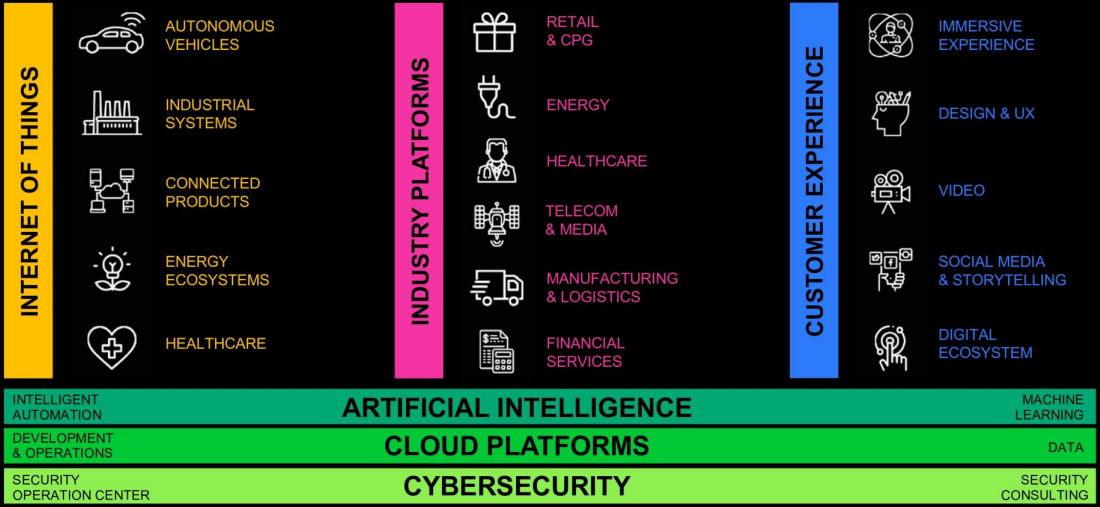
\includegraphics[width=0.5\linewidth]{images/bis2.png}
    \caption{Reply services}
\end{figure}
\noindent Reply provides end-to-end solutions for businesses looking to transform raw data into valuable insights. 
From data collection to advanced analytics, our approach ensures that companies can harness the full potential of their data.

In a consulting firm, professionals progress through several key roles, each with increasing responsibility and expertise:
\begin{enumerate}
    \item \textit{Consultant or analyst}: this is the entry-level position, where individuals focus on data analysis, research, and supporting senior consultants. 
        It's a foundational role that helps develop problem-solving, analytical, and research skills.
    \item \textit{Senior consultant or associate}: at this stage, professionals take on greater responsibility, leading specific project components and engaging more directly with clients.
        They begin to build deep expertise in a particular industry or domain while honing their client management skills.
    \item \textit{Manager}: managers oversee project teams, ensuring smooth project delivery while maintaining client relationships. 
        They are also involved in business development and sales. 
        This role emphasizes leadership, project management, and strategic client engagement.
    \item \textit{Senior manager}: with a broader scope, senior managers oversee multiple clients, contribute to business strategy, and play a key role in client acquisition. 
        Their focus shifts towards strategic thinking, high-level client management, and business development.
    \item \textit{Partner}: as part of the firm's leadership, partners are responsible for setting strategic direction, expanding business opportunities, and managing client relationships at the highest level.
        They bring extensive experience in business strategy, leadership, and client management.
\end{enumerate}

\subsection{Working models}
Consulting firms typically engage with clients through different contract models, depending on the project's nature and requirements.
\begin{itemize}
    \item \textit{Time and material}: in this model, the client pays based on the actual time spent and materials used, with an agreed hourly or daily rate for the resources employed. 
        This approach offers flexibility to adjust project requirements as work progresses and is well-suited for projects where specifications may evolve or are not fully defined at the outset. 
        However, budgeting can be challenging since the final cost depends on actual time and resources used.
    
    \item \textit{Turnkey}: the consulting provider takes full responsibility for delivering a complete and functional product or service. 
        The client receives the final result without managing the development process. 
        Costs and timelines are clearly defined, as the provider oversees all project phases. 
        This model requires minimal client involvement in day-to-day operations but offers limited flexibility to make changes once the project is underway.
        It is typically more expensive, as the provider factors in risks and contingencies.
    \item \textit{Service}: the client pays for a predefined set of consulting services, such as technical support, strategic guidance, or other specialized expertise. 
        This model allows clients to access specific skills without committing to a full project and is ideal for ongoing consultation or long-term support needs. 
        However, it may require clear agreements on service scope and expectations and is less suitable for projects with well-defined and temporary objectives.
\end{itemize}
\noindent The choice between these models depends on the project's complexity, flexibility needs, and budget considerations.
While time and material offers adaptability, turnkey ensures an end-to-end solution, and service contracts provide specialized expertise on demand.

\subsection{Key Performance Indicators}
\begin{definition}[\textit{Revenue}]
    The revenue is the total income generated by the company from its consulting services before any expenses are deducted.
\end{definition}
\noindent It is a key indicator of overall sales performance and business growth. 
In a consulting firm, revenue typically comes from client contracts and project fees.

\begin{definition}[\textit{Earning before tax}]
    Earning before tax is a financial metric that measures a company's profitability before accounting for income tax expenses.
\end{definition}
\noindent Earning before tax reflects the profit generated from core operations and other activities, such as investments or interest income, before taxes are deducted.

\begin{definition}[\textit{Cost on revenues}]
    cost on revenues is the ratio of costs directly associated with generating revenue, expressed as a percentage of total revenue.
\end{definition}
\noindent This metric helps assess how much of the revenue is consumed by costs such as consultant salaries, software tools, and travel expenses. 
A high cost-to-revenue ratio may indicate inefficiencies in service delivery or pricing strategies.

\begin{definition}[\textit{Unallocation}]
    Unallocation refers to staff who are not directly assigned to revenue-generating activities. 
\end{definition}
\noindent Monitoring unallocated costs is crucial for identifying inefficiencies and ensuring that expenses are properly distributed across projects and services.

\subsection{Project development}
The two main approaches used in project development are waterfall and agile, each with its own strengths and limitations.

\paragraph*{Waterfall}
The Waterfall model follows a sequential process, where each phase—analysis, design, development, testing, and implementation. 
Once a phase begins, changes to requirements are difficult to implement. 
This approach is best suited for projects with well-defined requirements from the start.
In consulting, waterfall is ideal for projects with stable and predetermined requirements, particularly in industries where compliance, documentation, and structured processes are essential.
\renewcommand*{\arraystretch}{1.5}
\begin{table}[!ht]
    \centering
    \begin{tabular}{|c|p{10cm}|}
    \hline
    \multicolumn{2}{|c|}{\textbf{Advantages}} \\ \hline
    \textit{Clear requirements}              & A well-defined project scope ensures a structured development process  \\ \hline
    \textit{Predictability}                  & Fixed timelines and structured phases make planning and resource allocation more manageable \\ \hline
    \textit{Comprehensive documentation}     & Each phase includes detailed documentation, providing a thorough project record \\ \hline
    \multicolumn{2}{|c|}{\textbf{Disadvantages}} \\ \hline
    \textit{Limited flexibility}             & Adapting to changes mid-project is challenging, making it less suitable for evolving requirements \\ \hline
    \textit{Delayed feedback}                & Since testing happens at the end, user feedback may come too late, requiring costly revisions \\ \hline
    \textit{Minimal client involvement}      & Limited collaboration during development can lead to misaligned expectations \\ \hline
\end{tabular}
\end{table}
\renewcommand*{\arraystretch}{1}

\paragraph*{Agile}
Agile follows an iterative and incremental approach, allowing for greater flexibility. 
Work is organized into sprints, each delivering a working product increment. 
Agile encourages continuous client collaboration and adapts easily to changing requirements.
In consulting, agile is well-suited for projects where requirements may evolve, or when quick, tangible results are needed.
\renewcommand*{\arraystretch}{1.5}
\begin{table}[!ht]
    \centering
    \begin{tabular}{|c|p{10cm}|}
    \hline
    \multicolumn{2}{|c|}{\textbf{Advantages}} \\ \hline
    \textit{Adaptability}                    & Changes can be accommodated at any stage, making Agile ideal for dynamic projects  \\ \hline
    \textit{Continuous feedback}             & Regular iterations ensure alignment with user needs and expectations \\ \hline
    \textit{Client collaboration}            & Ongoing client involvement fosters a more interactive and responsive development process\\ \hline
    \multicolumn{2}{|c|}{\textbf{Disadvantages}} \\ \hline
    \textit{Uncertain timeline}              &  Iterative cycles can introduce unpredictability, making planning and resource management more complex \\ \hline
    \textit{Minimal documentation}           & Agile prioritizes working software over documentation, which may be a drawback in highly regulated industries\\ \hline
    \textit{Scope creep}                     & Frequent changes and added features can lead to uncontrolled project expansion if not properly managed\\ \hline
\end{tabular}
\end{table}
\renewcommand*{\arraystretch}{1}